\documentclass{article}
\usepackage{tikz}
\usepackage{tkz-euclide} % loads  TikZ and tkz-base
%\usetkzobj{all}
\usetikzlibrary{calc,math}
\begin{document}


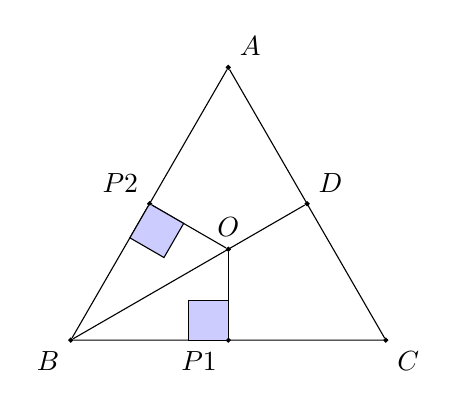
\begin{tikzpicture}
[scale=2,>=stealth,point/.style={draw,circle,fill = black,inner sep=0.5pt},]

%Triangle sides




%Labeling points
\node (A) at (1,1.732)[point,label=above right:$A$] {};
\node (B) at (0, 0)[point,label=below left:$B$] {};
\node (C) at (2, 0)[point,label=below right:$C$] {};
\node (O) at (1,0.577)[point,label=above:$O$] {};
\node (D) at (1.5,0.866)[point,label=above right:$D$] {};
\node (P1) at (1,0)[point,label=below left:$P1$] {};
\node (P2) at (0.5,0.866)[point,label=above left:$P2$] {};

%Drawing triangle ABC
\draw (A) -- node[left] {$\textrm{}$} (B) -- node[below] {$\textrm{}$} (C) -- node[above,xshift=5mm] {$\textrm{}$} (A);


%Joining BD
\draw (B)--(D);
\draw (O)--(P1);
\draw (O)--(P2);

%Drawing and marking angles
%\tkzMarkAngle[fill=orange!10,mark=||](D,B,A)
%\tkzMarkAngle[fill=orange!10,mark=||](C,B,D)
%\tkzMarkAngle[fill=green!40,size=0.5cm,mark=](A,B,C)
\tkzMarkRightAngle[fill=blue!20](O,P1,B)
\tkzMarkRightAngle[fill=blue!20](O,P2,B)
%\tkzLabelAngle[pos=0.25](D,B,A){$\theta$}
%\tkzLabelAngle[pos=0.25](C,B,D){$\theta$}
%\tkzLabelAngle[pos=0.65](A,B,C){$\alpha$}


\end{tikzpicture}
\end{document}
